%!TEX root = ../TAMUTemplate.tex
%%%%%%%%%%%%%%%%%%%%%%%%%%%%%%%%%%%%%%%%%%%%%%%%%%%
%
%  New template code for TAMU Theses and Dissertations starting Fall 2016.
%
%  Author: Sean Zachary Roberson 
%	 Version 3.08.16
%  Last updated 8/19/2016
%
%%%%%%%%%%%%%%%%%%%%%%%%%%%%%%%%%%%%%%%%%%%%%%%%%%%

%%%%%%%%%%%%%%%%%%%%%%%%%%%%%%%%%%%%%%%%%%%%%%%%%%%%%%%%%%%%%%%%%%%%%%
%%                           SECTION I
%%%%%%%%%%%%%%%%%%%%%%%%%%%%%%%%%%%%%%%%%%%%%%%%%%%%%%%%%%%%%%%%%%%%%


\pagestyle{plain} % No headers, just page numbers
\pagenumbering{arabic} % Arabic numerals
\setcounter{page}{1}


\chapter{\uppercase {Introduction}}

On July 4th, 2012 when the long predicted Higgs boson (H) was discovered by both the ATLAS~\cite{20121} and CMS~\cite{201230} collaborations at the European Organization for Nuclear Research (CERN).
It took almost 50 years for experimentalists to confirm the existence of the boson first proposed in 1964 to give mass to itself and all of the other massive particles through the process of electroweak symmetry breaking.
Using 19.6\fbinv of 8\tev data from the Compact Muon Solenoid (CMS) experiment at CERN, the Higgs boson mass was measured to be \longmass{125.7}{0.3}{0.3}{\gev} by five major decay modes: $H\rightarrow\gamma\gamma$, $H\rightarrow\tau\tau$, $H\rightarrow{bb}$, $H\rightarrow{ZZ}$, and $H\rightarrow{WW}$~\cite{CMS-PAS-HIG-13-005}.
Every property of the new boson and all of its decay channels must be studies in great detail to confirm that it is indeed the SM Higgs boson and not a very similar particle.
Currently the properties of the new boson are consistent with those predicted by the SM, but any deviation from the SM predictions could point to some new, as yet unexplored physics.

\begin{figure}[bt]
	\centering
	\begin{subfigure}[t]{0.415\textwidth}
		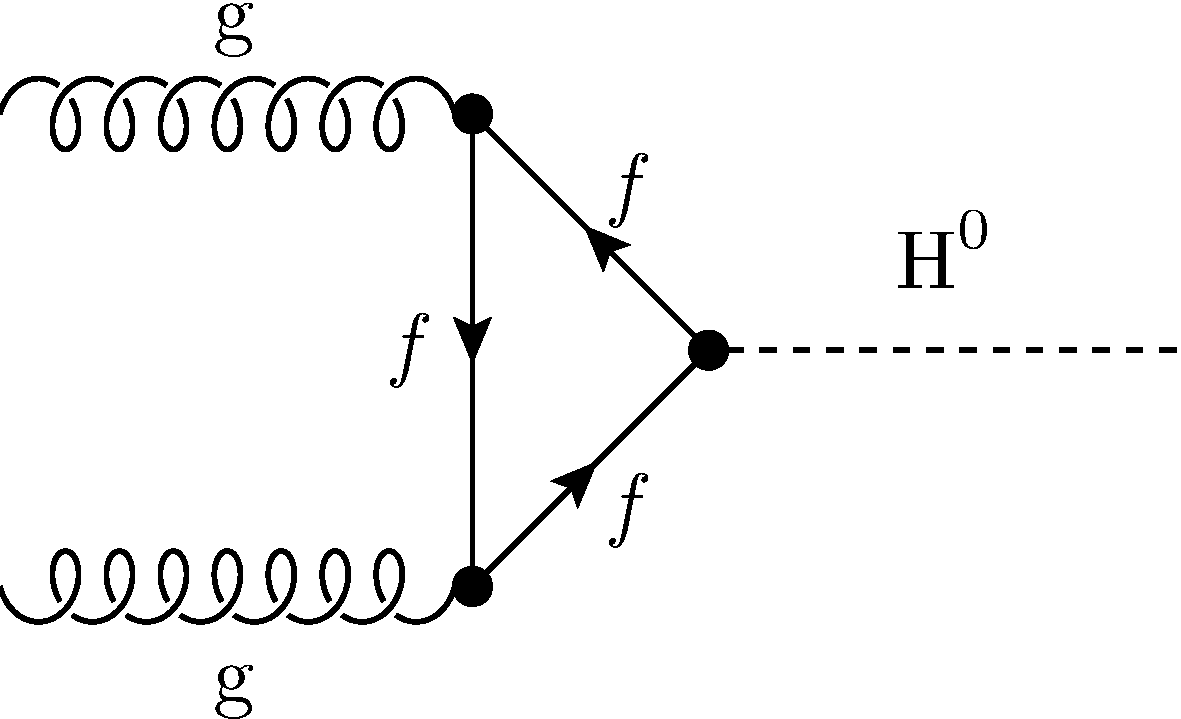
\includegraphics[width=\textwidth]{\figpath/FeynmanDiagrams/ggH.eps}
		\label{fig:ggH}
	\end{subfigure}%
	\begin{subfigure}[t]{0.415\textwidth}
		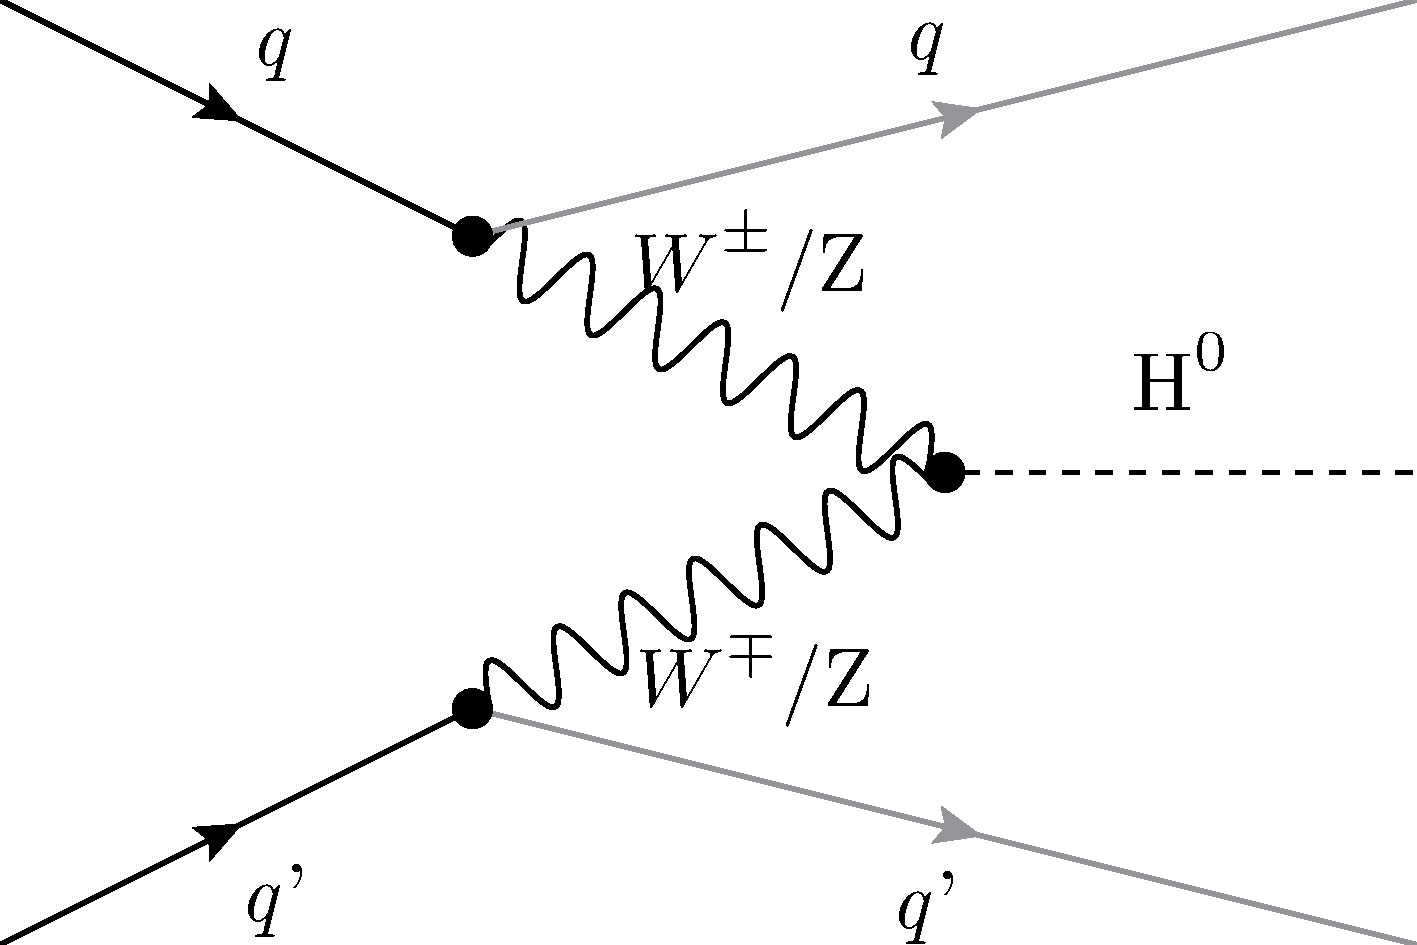
\includegraphics[width=\textwidth]{\figpath/FeynmanDiagrams/qqH.eps}
		\label{fig:qqH}
	\end{subfigure}

	\begin{subfigure}[t]{0.415\textwidth}
		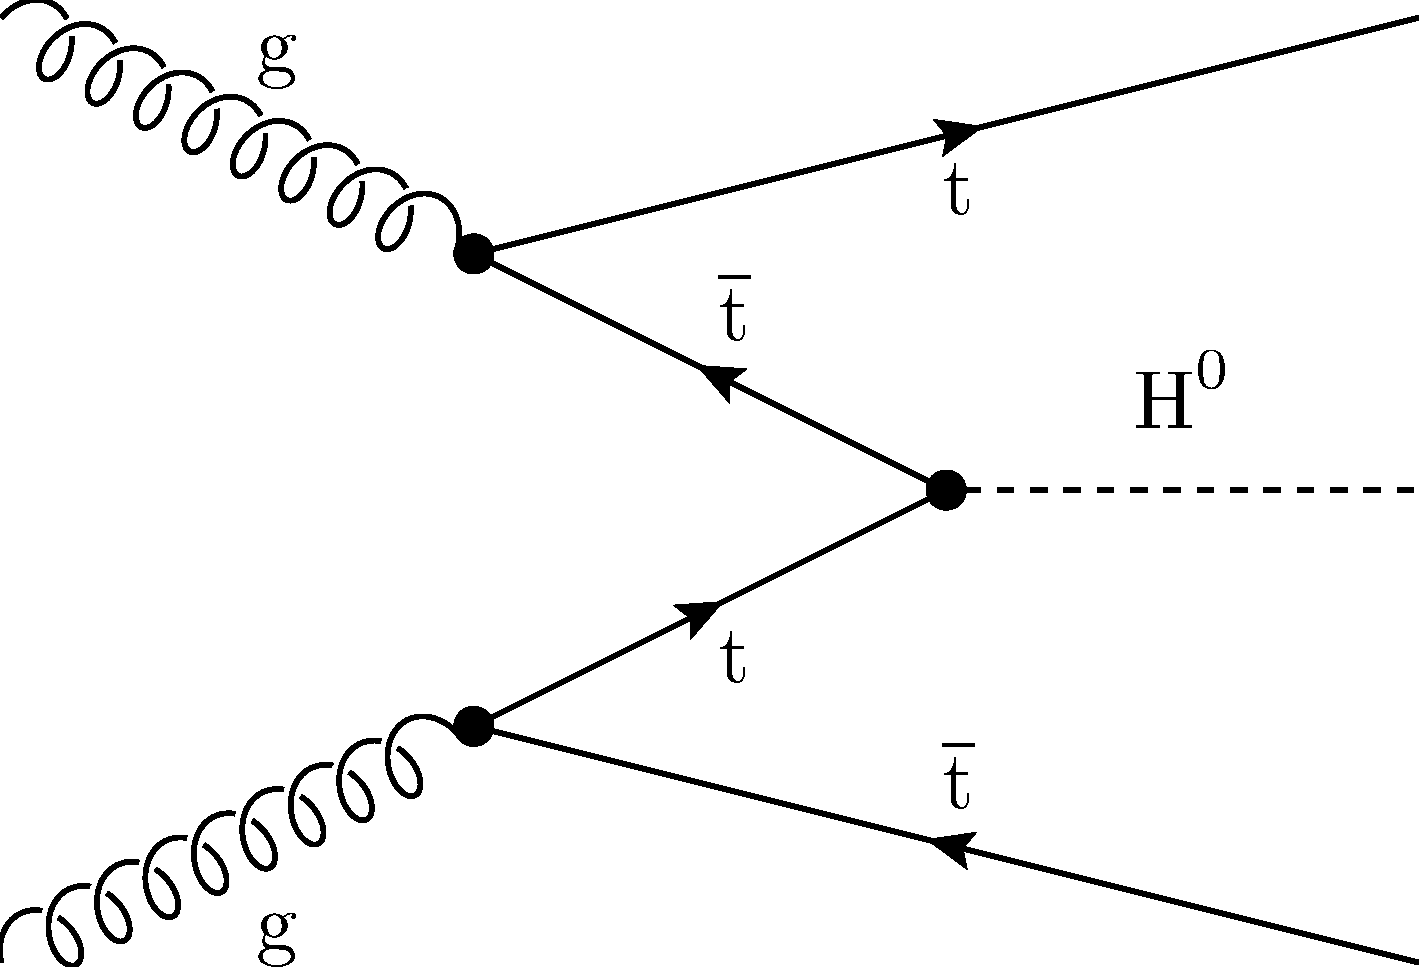
\includegraphics[width=\textwidth]{\figpath/FeynmanDiagrams/ttH.eps}
		\label{fig:ttH}
	\end{subfigure}%
	\begin{subfigure}[t]{0.415\textwidth}
		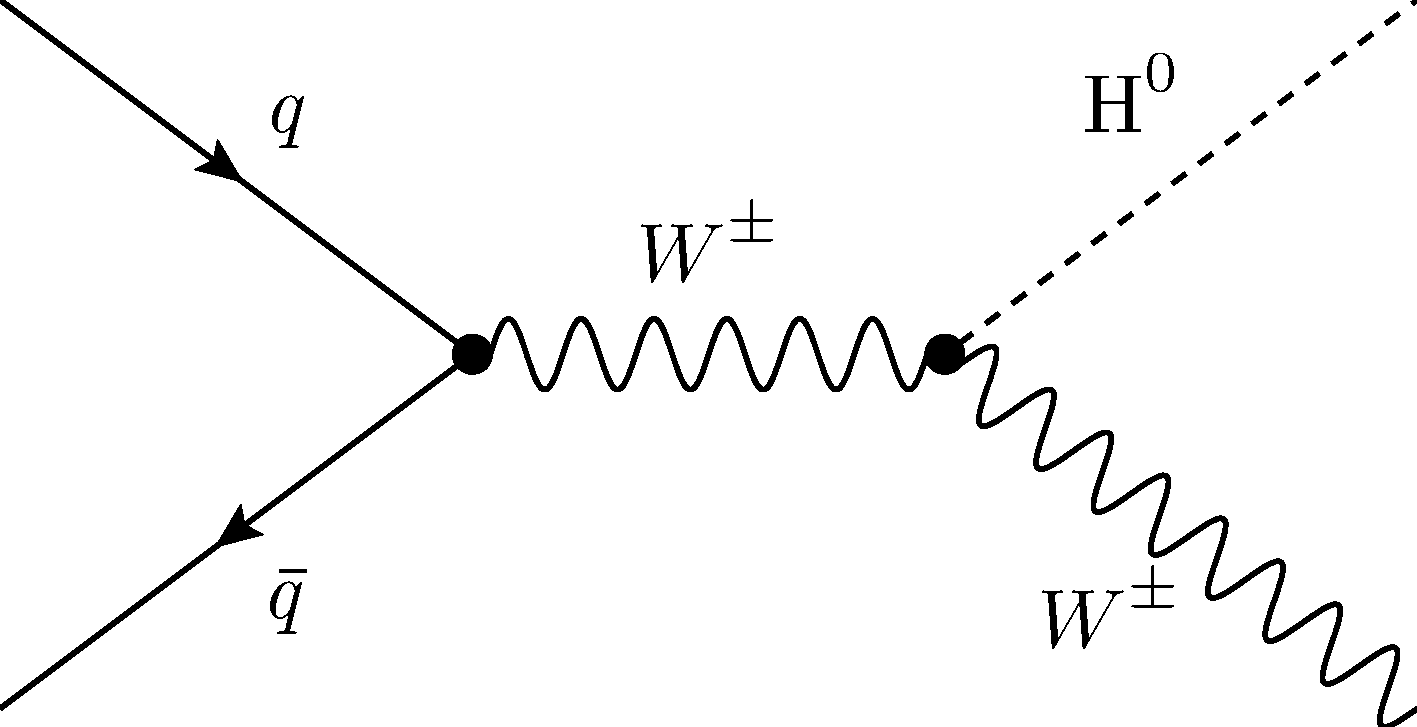
\includegraphics[width=\textwidth]{\figpath/FeynmanDiagrams/WH.eps}
		\label{fig:WH}
	\end{subfigure}
	\caption{Feynman diagrams for the four Higgs production mechanisms with associated $l{\nu}qq$ decays: gluon-gluon fusion (upper left), vector-boson fusion (upper right), \ttbar fusion (lower left), and associated production (lower right).}
	\label{fig:Higgs_WW_lnujj_feynman}
\end{figure}

\begin{figure}[!hbt]
	\centering
	\begin{subfigure}[t]{0.54\textwidth}
		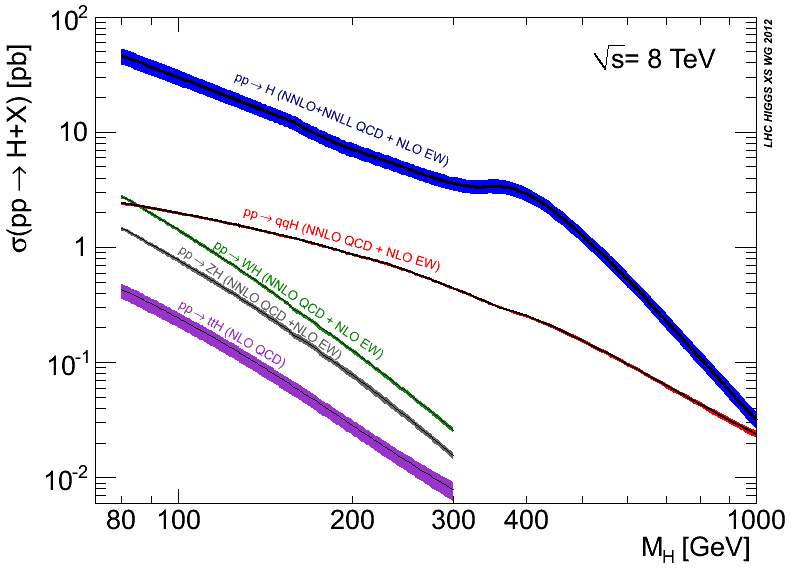
\includegraphics[width=\textwidth]{\figpath/Chapter1/Higgs_XS_8TeV.png}
		\label{fig:CERN_accelerator_complex}
	\end{subfigure}
	\begin{subfigure}[t]{0.41\textwidth}
		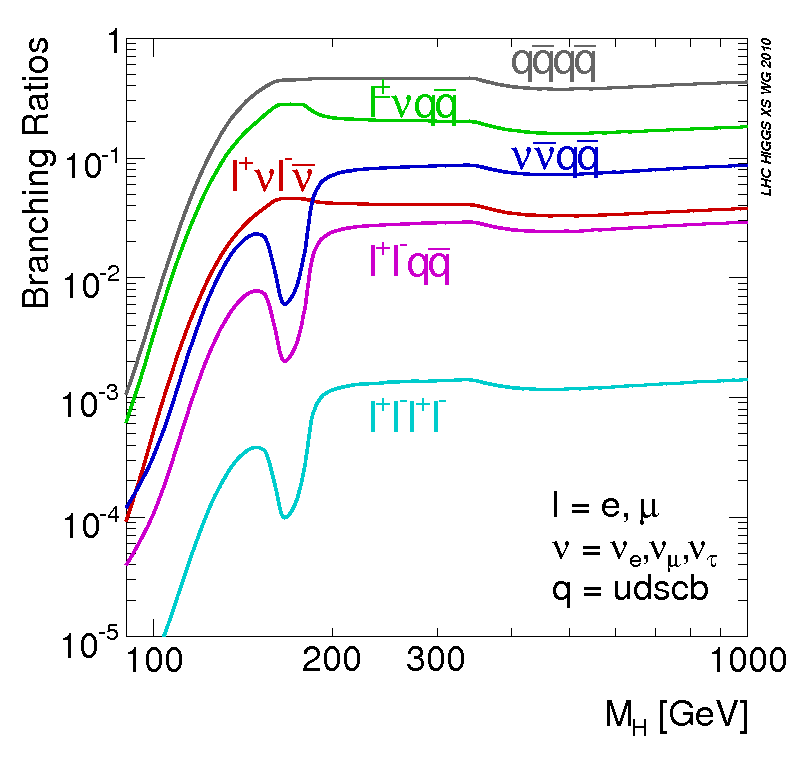
\includegraphics[width=\textwidth]{\figpath/Chapter1/Higgs_BR_4fermion.png}
		\label{fig:LHC_LEP_injection_complex}
	\end{subfigure}
	\caption{The Standard Model Higgs production cross sections at 8\tev (left) and WW branching ratios to four fermion final states (right).}
	\label{fig:Higgs_XS_and_BR}
\end{figure}

To this end, this analysis will use the \HWWlnujj decay channel, as seen in figure~\ref{fig:Higgs_WW_lnujj_feynman}, to search for a 125\gev Higgs boson.
Although the \HWWlnujj channel was used in the original combined limit, the previous search was not sensitive to the ``low mass'' Higgs, but only to a $\MH>170\gev$~\cite{CMS-PAS-HIG-13-027}.
While at 125\gev the gluon-gluon fusion (ggF) production cross section\footnote{This analysis is independent of production mode, but selects for a specific decay channel.} and $l\nu{qq}$ branching ratio are high, as seen in figure~\ref{fig:Higgs_XS_and_BR}, there are significant experimental challenges to overcome.
Because the Higgs mass is less than two times the mass of the W boson, at least on of the W must be created off-shell.
On top of that, the presence of a neutrino makes it a challenge to fully reconstruct the initiating particle.
For these reasons the $WW\rightarrow{l\nu}{l\nu}$ decay channel was the most sensitive of the $WW$ channels during the 2012 combination.
My proposal is to search for the low mass Higgs boson in the semi-leptonic channel using a matrix element (ME) technique to boost the sensitivity.
